\documentclass{article}
\usepackage{pgfplots}
\usetikzlibrary{matrix}

\begin{document}

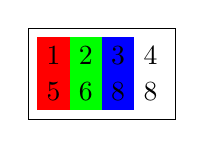
\begin{tikzpicture}

\tikzstyle{mymatrix}=[draw]
\foreach \c [count=\i] in {red, green, blue} {
    \globaldefs=1
    \edef\dotikzset{
        \noexpand\tikzset{
            mymatrix/.append style={
                column \i/.style={
                    nodes={fill=\c}
                }
            }
        }
    }
    \dotikzset
}

\matrix (m) [matrix of nodes, mymatrix] {
 1 & 2 & 3 & 4 \\
 5 & 6 & 8 & 8 \\ };

\end{tikzpicture}

\end{document}
